\flushleft
\section{Interpretation sur $ \alpha $ and $ \beta $ Intensification et diversification}

Avec $ \alpha $ = 0, seul la \textit{heuristic information} est prise en compte; la ville la plus proche est donc choisie \`a chaque pas. Au contraire, avec $ \beta = 0 $, seules l'intensit\'ee de ph\'eromone jouent. on peut voir ci dessous les r\'esultat si on donne \`a $ \alpha = 0 $ et $ \beta = 5 $\\

\begin{figure}[H]
% 1st minipage
\begin{minipage}[t]{0.5\linewidth}
\centering
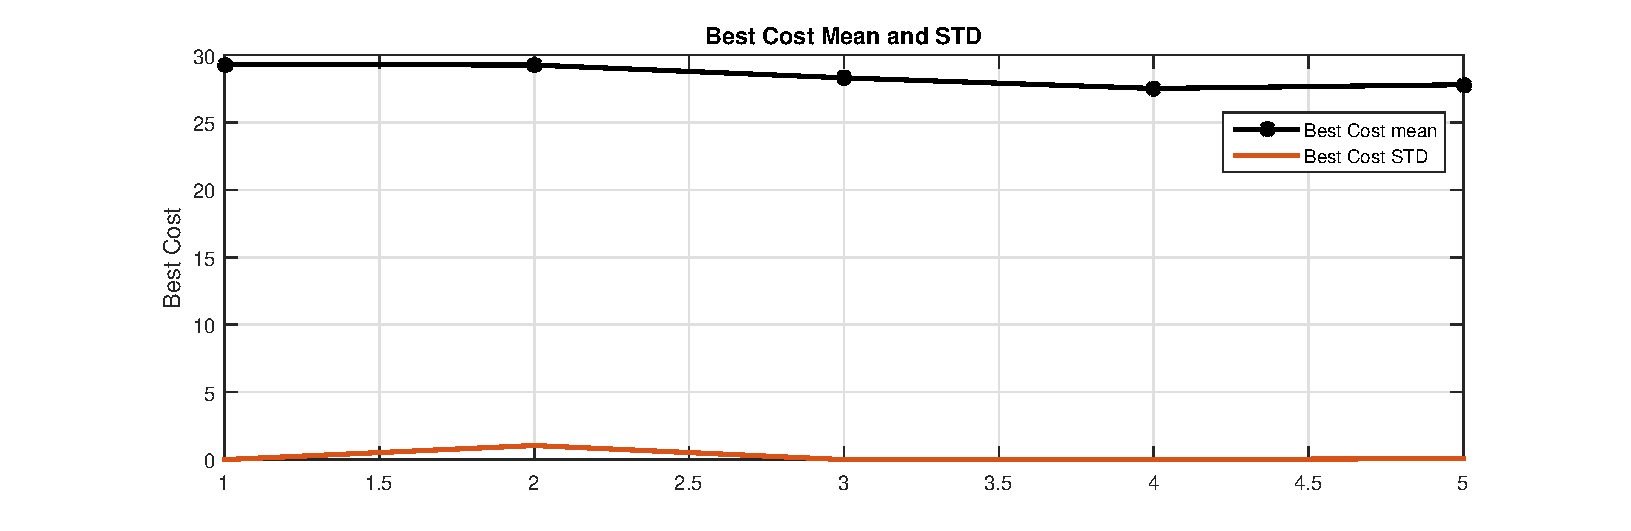
\includegraphics[width=\linewidth]{../figures/exp_alpha_0/BestCost_meanANDstd.eps}
\caption{Mean and STD variation of Best Cost $ \alpha=0 $}
\label{fig:exp_alpha_0_BestCost_meanANDstd}
\end{minipage}
% 2nd minipage
\hspace{2mm}
\begin{minipage}[t]{0.5\linewidth}
\centering
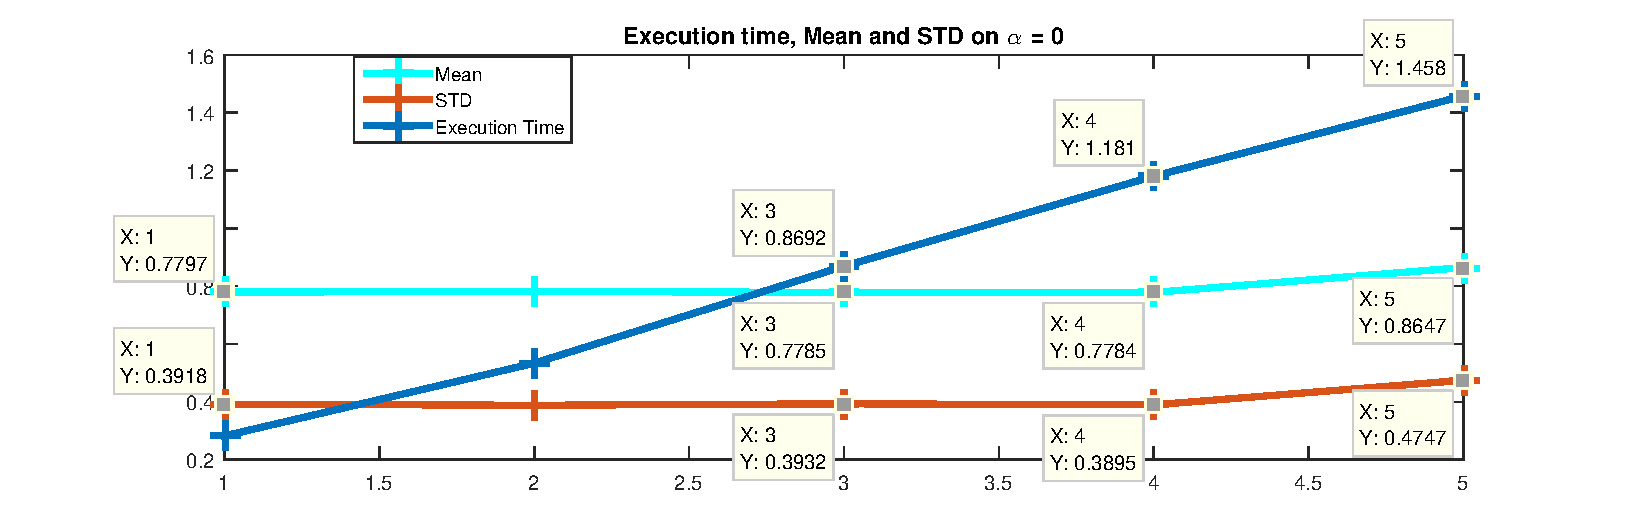
\includegraphics[width=\textwidth]{../figures/exp_alpha_0/AS_ExecTimeMeanAndSTD.eps}
\caption{Execution time, Mean and STD on $ \alpha = 0 $}
\label{fig:exp_alpha_0_AS_ExecTimeMeanAndSTD}
\end{minipage}
\end{figure}
Alors pour \'eviter une s\'election trop rapode d'un trajet, un compromis entre ces deux param\'etres, jouant sur les comportements de \textit{diversification} et d'\textit{intensification} est n\'ecessaire.

$ \alpha $ et $ \beta $ d\'eterminent l'influence relative des pistes de ph\'eromone et de l'information heuristique.\\
plus la valeur de $ \alpha $ sera \'elev\'e plus l'\textit{intensification} sera importante, car plus les pistes auront une influence sur le choix des fourmis. \`A l'inverse, plus $ \alpha $ sera faible, plus la \textit{diversification} sera forte car les fourmis \'evitront les pistes.
	$ \beta $ agit de fa\c{c}on laire. On doit donc g\'erer \'a la fois les deux param\`etres pour r\'egler ces aspects. et ci dessous les r\'esultats confirme ce qu'on dit
\begin{figure}[H]
% 1st minipage
\begin{minipage}[t]{0.5\linewidth}
\centering
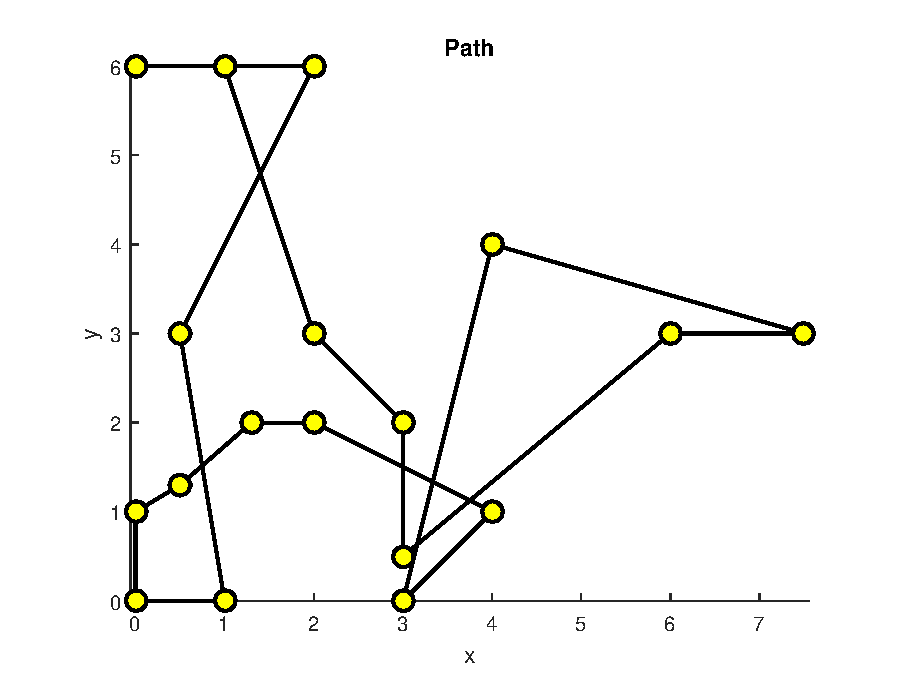
\includegraphics[width=\linewidth]{../figures/exp_alpha_0_beta_1/pathbigfig.eps}
\caption{Path avec diminution de la valuer de $ \beta=1 $}
\label{fig:exp_alpha_0_beta_1_pathbigfig}
\end{minipage}
% 2nd minipage
\hspace{2mm}
\begin{minipage}[t]{0.5\linewidth}
\centering
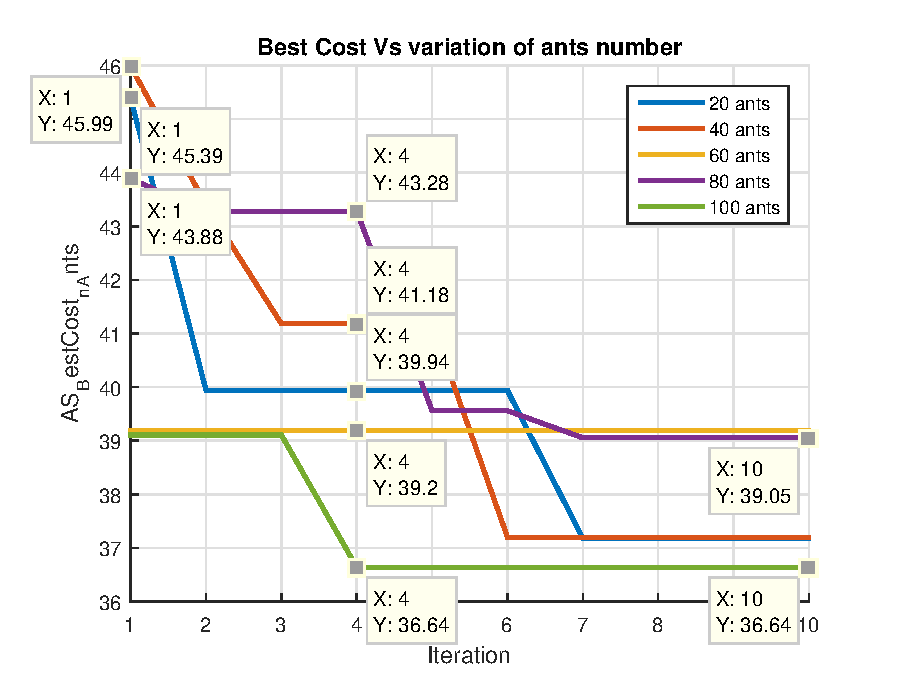
\includegraphics[width=\textwidth]{../figures/exp_alpha_0_beta_1/AS_BestCost_n_Ants.eps}
\caption{Best Cost with ants variation$ \beta=1$ $ \alpha=0 $}
\label{fig:exp_alpha_0_beta_1_AS_BestCost_n_Ants}
\end{minipage}
On peut bien remarque l'influence du changement de la valeur de $ \beta $ quand par comparaison avec $ \beta=5 $.
\end{figure}